\documentclass[12pt,a4paper,notitlepage,twoside]{article}
\usepackage{polski}
\usepackage[utf8]{inputenc}
\usepackage{mathtools}
\usepackage{helvet}
\usepackage[top=2.5cm, bottom=2.5cm, left=3cm, right=2.5cm]{geometry}
\usepackage{graphicx}
\usepackage[absolute]{textpos}
\usepackage{tocloft}
\usepackage{cite}
\usepackage[numbib,notlof,notlot,nottoc]{tocbibind}
\usepackage{indentfirst}
\usepackage{fancyvrb}
\usepackage{listings}
\usepackage{float}
\linespread{1.3}

\renewcommand{\cftsecleader}{\cftdotfill{\cftdotsep}}
\renewcommand\figurename{Rys.}
%% \setlength\cftparskip{-2pt}
\setlength\cftbeforesecskip{1pt}
\setlength\cftaftertoctitleskip{2pt}

\lstset{
  numbers=left,
  breaklines=true,
  captionpos=b,
  language=C++,
  xleftmargin=\parindent,
  basicstyle=\small,
  inputencoding=utf8,
  escapeinside={\%*}{*)}
}

\usepackage{hyperref}
\hypersetup{
  colorlinks=true, %set true if you want colored links
  linktoc=all,     %set to all if you want both sections and subsections linked
  linkcolor=black,  %choose some color if you want links to stand out
  citecolor=black,
  urlcolor=black,
}

\setlength{\TPHorizModule}{10mm}
\setlength{\TPVertModule}{\TPHorizModule}
\textblockorigin{30mm}{25mm}

\makeatletter

\renewcommand{\maketitle}{\begin{titlepage}

    \begin{center}
      
\includegraphics[width=2.5cm]{img/polsl-logo}
    \end{center}

    \vspace{0.5cm}
    \begin{center}
      \Large{\textbf{\textsc{Politechnika Śląska\\
	    Wydział Automatyki, Elektroniki i Informatyki\\
	    Kierunek Informatyka\\}}}
    \end{center}

    \vspace{0.5cm}
    \begin{center}
      \Large{Projekt inżynierski}
    \end{center}

    \begin{center}

      \vspace{0.5cm}
      {\fontsize{30}{36}\selectfont \@title}

    \end{center}

    \begin{textblock}{10}(0,19)
      \noindent{\fontsize{14}{21}{Autor: \@author\\
	  Kierujący pracą: dr inż. Zbigniew Szaszkowski}}
    \end{textblock}
    \begin{textblock}{15.5}(0,24)
      \begin{center}
	Gliwice, czerwiec 2015
      \end{center}
    \end{textblock}
  \end{titlepage}

}

\makeatother

\author{Marcin Kolny}

\title{Rozpoznawanie ciągów znaków z wykorzystaniem metod segmentacji obrazu}

\begin{document}

\maketitle
\newpage
\tableofcontents
\newpage
\section{Analiza obrazu}
\subsection{Podstawowe informacje dotyczące przetwarzania obrazów}
\subsubsection{Tryb koloru}
Określenie sposobu reprezentacji kolorów w obrazach rastrowych nazywamy \textbf{trybem koloru}. Wyróżniamy następujące tryby koloru:
\begin{itemize}
  \item czarno-biały - w obrazie występują tylko kolory: biały i czarny,
  \item skala szarości - oprócz koloru czarnego i białego, występuje cała gama jasności pośrednich,
  \item tryb kolorowy - piksele mają przyporządkowane kolory z przestrzeni barw.
\end{itemize}
Symbolem $I$ będziemy oznaczać zbiór kolorów. Dla trybu czarno-białego
\begin{gather*}
  I = \{0, 1\}
\end{gather*} gdzie 0 reprezentuje kolor czarny, a 1 kolor biały.\\
Dla trybu skali szarości
\begin{gather*}
  I = \{0, 1, ..., 2^b-1\}
\end{gather*}
gdzie $b$ jest liczbą bitów potrzebnych do reprezentacji jasności, 0 oznacza kolor czarny, $2^b-1$ kolor biały, a pozostałe wartości opisują jasność koloru. Najczęściej wartość $b$ jest wielokrotnością liczby 8.\\
Dla trybu kolorowego
\begin{gather*}
  I = I_1 \times I_2 \times ... \times I_n,
\end{gather*}
gdzie
\begin{gather*}
  I_1 = I_2 = ... = I_n = \{0, 1, ..., 2^b-1\}
\end{gather*}
oraz $n\in \mathbb{N} \wedge n > 1$ jest liczbą kanałów z przestrzeni barw. \\
Dla przestrzeni barw RGB
\begin{gather*}
  I = I_R \times I_G \times I_B
\end{gather*}
gdzie $I_R$, $I_G$, $I_B$ oznaczają odpowiednio jasność kolorów czerwonego, zielonego i niebieskiego. Przestrzeń RGB jest trzykanałowa.
\subsubsection{Obraz cyfrowy}
Obraz cyfrowy definiujemy jako funkcję
\begin{gather*}
  f: \{0, 1, ..., N-1\} \times \{0, 1, ..., M-1\} \rightarrow I,
\end{gather*}
gdzie $M$, $N$ oznaczają odpowiednio szerokość i wysokość obrazu.\\
Wartość funkcji $f(x, y)$ nazywamy \textbf{pikselem}.\\
Obrazy cyfrowe możemy podzielić ze względu na tryb opisu koloru:
\begin{itemize}
  \item czarno-białe,
  \item jednokanałowe (monochromatyczne),
  \item wielokanałowe (kolorowe).
\end{itemize}
Na rysunku~\ref{fig:image_examples} przedstawione zostały obrazy w których zastosowano wyżej wymienione tryby opisu koloru.\\
Symbolem $P_{N,M}$ będziemy oznaczać zbiór
\begin{gather*}
  P_{N,M} = \{0, 1, ..., N-1\} \times \{0, 1, ..., M-1\}.
\end{gather*}
Każdy obraz cyfrowy $P = (P_{N,M}; f; I)$ opisuje trójka\\
$P_{N,M}$ - zbiór współrzędnych punktów obrazu,\\
$I$ - zbiór opisujący kolor obrazu,\\
$f$ - funkcja przyporządkowująca punktowi kolor.

\begin{figure}
  \centering
  \begin{subfigure}[b]{0.45\textwidth}
    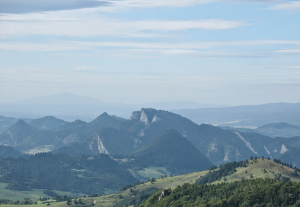
\includegraphics[width=\textwidth]{img/basics-image-color}
    \caption{Trzykanałowy obraz cyfrowy (kolorowy)}
    \label{fig:basics_image_color}
  \end{subfigure}
  ~
  \begin{subfigure}[b]{0.45\textwidth}
    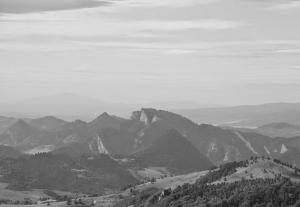
\includegraphics[width=\textwidth]{img/basics-image-gray}
    \caption{Jednokanałowy obraz cyfrowy (monochromatyczny)}
    \label{fig:basics_image_gray}
  \end{subfigure}
  ~
  \begin{subfigure}[b]{0.45\textwidth}
    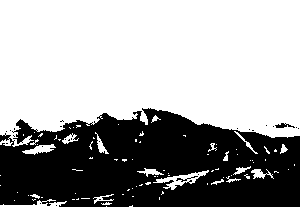
\includegraphics[width=\textwidth]{img/basics-image-binary}
    \caption{Obraz jednokanałowy (czarno-biały)}
    \label{fig:basics_image_binary}
  \end{subfigure}
  \caption{Obrazy cyfrowe wykorzystujące różne tryby kolorów}\label{fig:image_examples}
\end{figure}
\subsection{Podstawowe operacje przetwarzania obrazów}
Symbolem
\begin{gather*}
  P^{(in)} = (P_{N,M}^{(in)}, f^{(in)}, I^{(in)})
\end{gather*}
oznaczamy obraz wejściowy, a 
\begin{gather*}
  P^{(out)} = (P_{N,M}^{(out)}, f^{(out)}, I^{(out)})
\end{gather*}
obraz wyjściowy.

\subsubsection{Kadrowanie obrazu}
Operacja kadrowania polega na pozostawieniu na obrazie wejściowym tylko tych pikseli, które znajdują się w zdefiniowanym prostokątnym obszarze. Obraz wyjściowy po operacji kadrowania przyjmuje rozmiar obszaru, do którego kadrowany był obraz wejściowy.\\
Na rysunku~\ref{fig:crop_image} przedstawiona została operacja kadrowania obrazu. Celem kadrowania jest usunięcie z obrazu informacji, które są zbędne podczas wykonywania analizy obrazu, ponieważ mogą negatywnie wpłynąć na czas oraz rezultaty wykonania algorytmów.
\begin{figure}
  \centering
  \begin{subfigure}[b]{0.45\textwidth}
    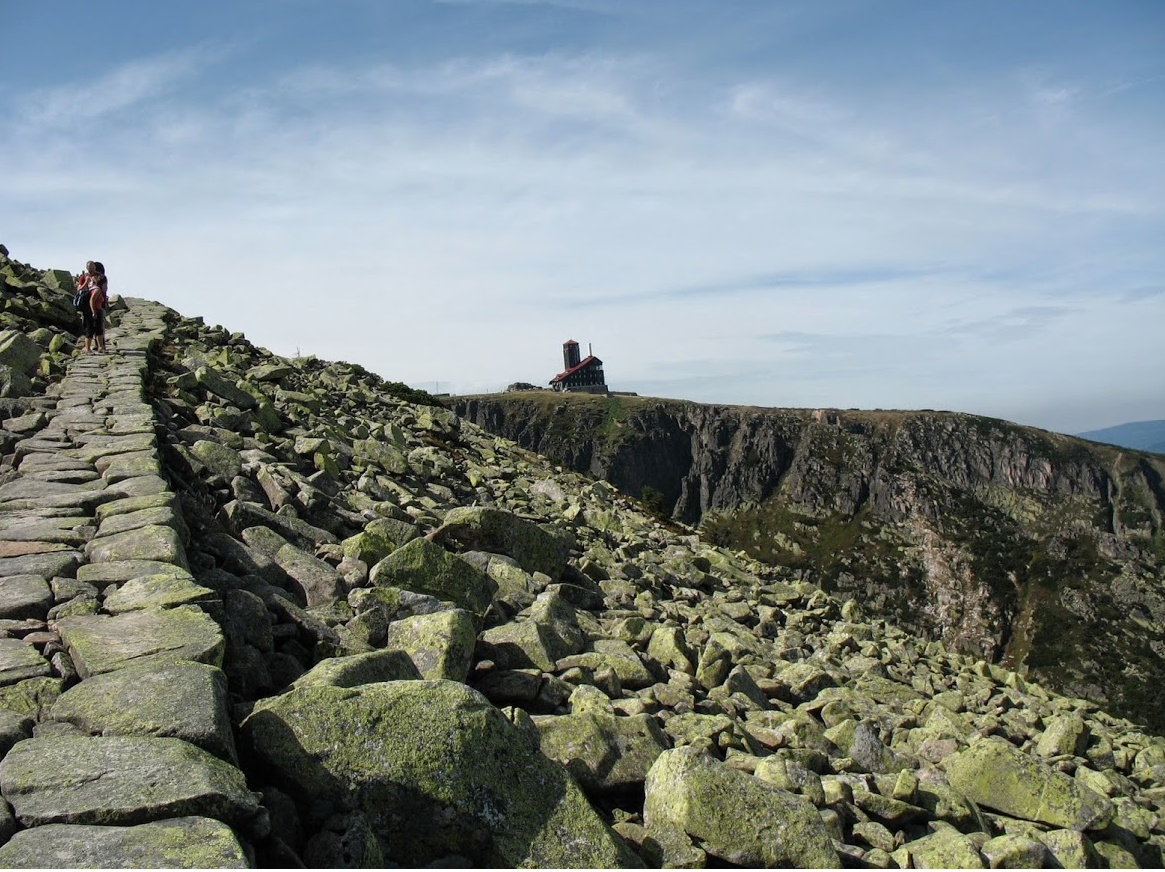
\includegraphics[width=\textwidth]{img/crop-image-before}
    \caption{Obraz wejściowy dla operacji kadrowania}
    \label{fig:crop_image_before}
  \end{subfigure}
  ~
  \begin{subfigure}[b]{0.45\textwidth}
    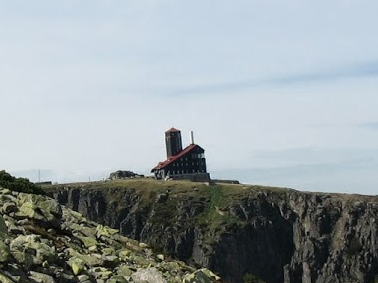
\includegraphics[width=\textwidth]{img/crop-image-after}
    \caption{Obraz wyjściowy, poddany operacji kadrowania}
    \label{fig:crop_image_after}
  \end{subfigure}
  \caption{Operacja kadrowania obrazu}\label{fig:crop_image}
\end{figure}
\subsubsection{Progowanie (binaryzacja)} \label{sssec:threshold}
Progowanie polega na podziale pikseli obrazu na dwie grupy, poprzez wybranie określonej wartości progowej $t$. Każdy piksel jest porównywany z wartością progową, i w zależności od tego, czy wartość piksela jest większa od wartości progowej, czy mniejsza, w tej samej pozycji nowo powstałego obrazu, przypisuje się wartość $1$, lub $0$. Operację można opisać wzorem:
\begin{gather*}
  f^{(out)}(x, y) = \left\{\begin{matrix}
  1, dla \: f^{(in)}(x, y) > t,\\
  0, dla \: f^{(in)}(x, y) \leq t,
  \end{matrix}\right. \quad (x, y) \in P^{(in)}_{N,M}
\end{gather*}
Na rysunku~\ref{fig:threshold_image} przedstawiony został wynik operacji progowania na przykładowym obrazie monochromatycznym.
\begin{figure}
  \centering
  \begin{subfigure}[b]{0.45\textwidth}
    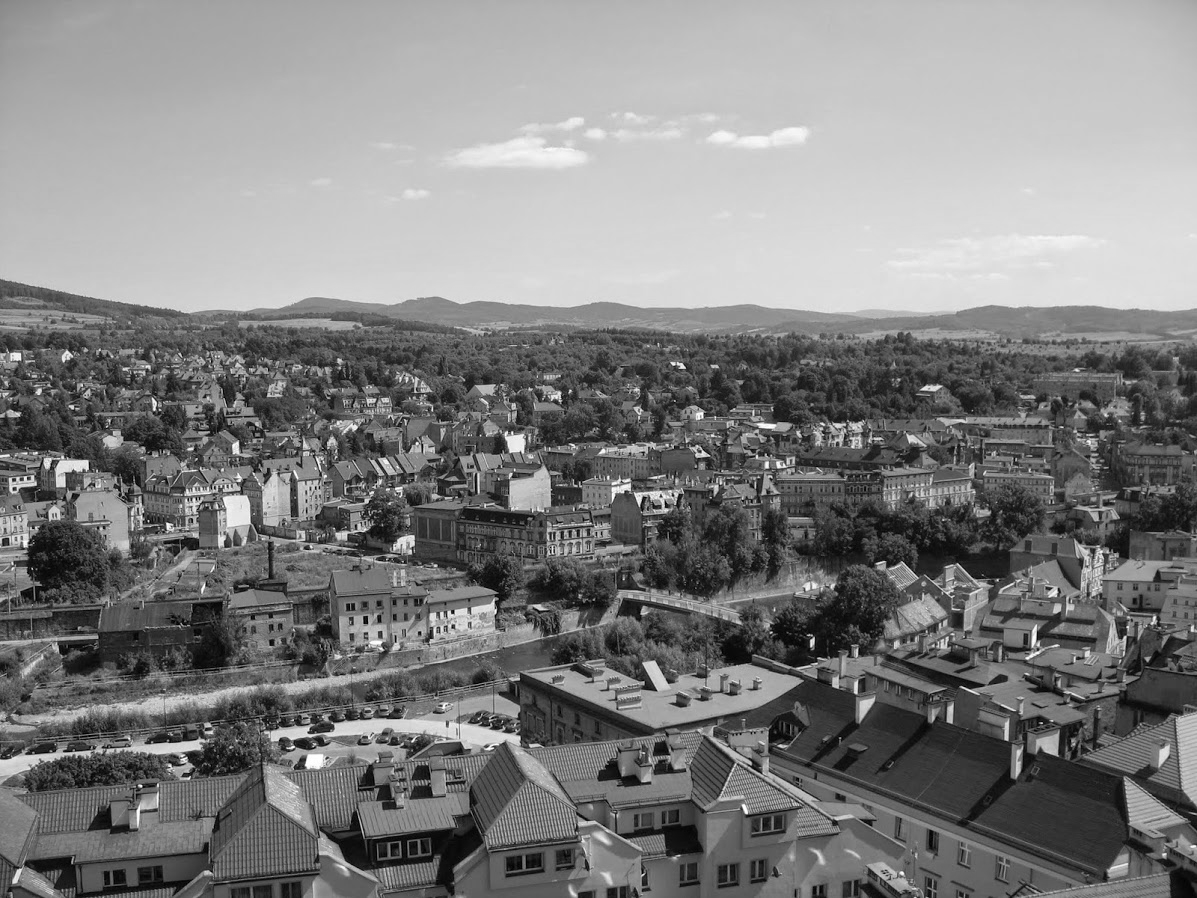
\includegraphics[width=\textwidth]{img/threshold-before}
    \caption{Obraz wejściowy dla operacji progowania}
    \label{fig:threshold_before}
  \end{subfigure}
  ~
  \begin{subfigure}[b]{0.45\textwidth}
    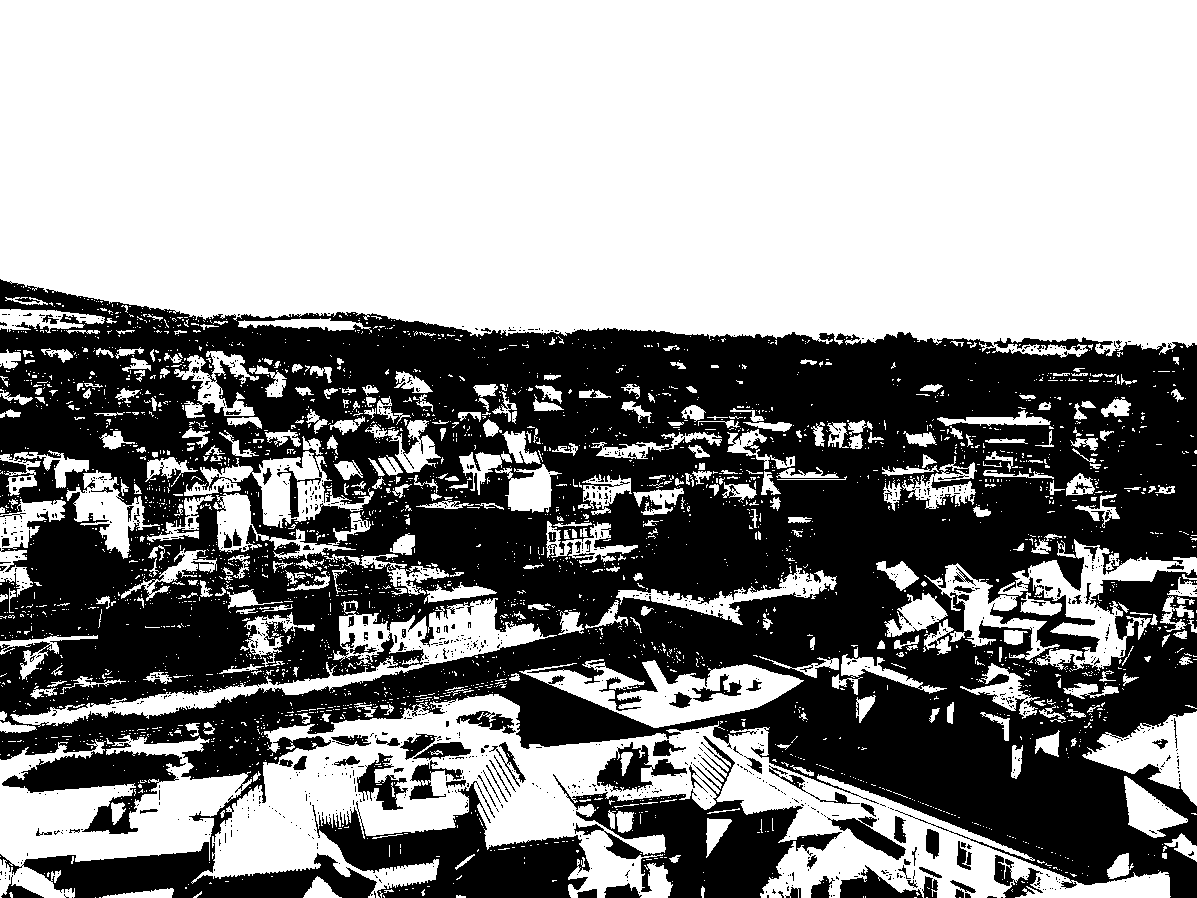
\includegraphics[width=\textwidth]{img/threshold-after}
    \caption{Obraz wyjściowy, poddany operacji progowania}
    \label{fig:threshold_after}
  \end{subfigure}
  \caption{Operacja progowania z wartością progu $t=128$ dla obrazu jednokanałowego}\label{fig:threshold_image}
\end{figure}

\paragraph{Progowanie obrazów wielokanałowych}\mbox{}\\
Zazwyczaj operacji progowania poddawane są obrazy jednokanałowe. Istnieje jednak możliwość wykonania operacji progowania dla obrazów wielokanałowych (np. dla obrazów RGB). Operacja ta definiowana jest następującym wzorem:
\begin{gather*}
  f^{(out)}(x, y) = \left\{\begin{matrix}
  1, \; \text{jeżeli} \; \forall c \in C, \; f^{(in)}(x, y, c) > t(c),\\
  0, \; \text{jeżeli} \; \exists c \in C, \; f^{(in)}(x, y, c) \leq t(c),
  \end{matrix}\right. \quad (x, y) \in P^{(in)}_{N,M} c=0,1,2,...,C,
\end{gather*}
gdzie $C$ to liczba kanałów w obrazie.
Algorytm progowania operujący na wielu kanałach może zostać wykorzystany, kiedy znana jest dokładna barwa badanego obiektu.

\paragraph{Progowanie lokalne}\mbox{}\\
Progowanie lokalne znajduje zastosowanie w przypadku gdy obraz jest niejednolicie oświetlony. Trudno jest dobrać globalny próg w taki sposób, aby wyekstrachować z obrazu nawet większość porządanych obiektów. Progowanie lokalne polega na wyznaczeniu danego progu w sąsiedztwie aktualnie przetwarzanego piksela. 
\begin{gather*}
  f^{(out)}(x, y) = \left\{\begin{matrix}
  1, dla \: f^{(in)}(x, y) > T(x, y),\\
  0, dla \: f^{(in)}(x, y) \leq T(x, y),
  \end{matrix}\right. \quad (x, y) \in P^{(in)}_{N,M},
\end{gather*}
gdzie $T(x, y)$ to funkcja zwracająca próg w zadanym sąsiedztwie piksela o współrzędnych $(x, y)$. Zwykle jako funkcję wyznaczania progu przyjmuje się wartość średnią lub sumą ważoną, wykorzystującą krzywą Gaussa.

\subsubsection{Filtracja obrazu}
Poprzez \textbf{jądro (maskę)} w kontekscie przetwarzania obrazów rozumiemy kształt którym parametryzowana jest operacja filtracji obrazu. Symbolami $k_N$, $k_M$ będę oznaczał rozmiar jądra (kolejno wysokość oraz szerokość).\\
Operacje filtracji mają na celu wykonanie zadanego przekształcenia matematycznego dla każdego piksela, generując tym samym nowy obraz. Filtrację obrazu stosuje się zwykle w celu wydobycia z obrazu żądanych informacji lub usunięcia szumu. Poniżej wymienionych zostało kilka najczęściej używanych operacji filtrowania obrazu:
\begin{itemize}
\item filtr uśredniający - stosowany jest w celu rozmycia obrazu
  \begin{gather*}
    f^{(out)}(x, y) = \frac{\sum\limits_{x=M-k_\frac{M}{2}}^{M+\frac{k_M}{2}} \sum\limits_{y=N-\frac{k_N}{2}}^{N+\frac{k_N}{2}} f^{(in)}(x, y)}{k_M \cdot k_N}, \quad (x, y) \in P^{(in)}_{N,M},
  \end{gather*}
\item filtr medianowy - wykorzystywany jest do usuwania zakłóceń na obrazie
  \begin{gather*}
    f^{(out)}(x, y) = mediana(\{f^{(in)}(x, y), \;x \in \big< M-\frac{k_x}{2}, M+\frac{k_x}{2}\big> \\
    \wedge\; y \in \big< N-\frac{k_y}{2}, N+\frac{k_y,}{2}\big>\}), \quad (x, y) \in P^{(in)}_{N,M},
  \end{gather*}
\item filtr Gaussa - podobnie jak filtr uśredniający, filtr Gaussa stosuje się do redukcji detali na obrazie poprzez jego rozmycie
  \begin{gather*}
    f^{(out)}(x, y) = \frac{1}{\sqrt{2 \pi \sigma}} e^{-\frac{x^2+y^2}{2 \sigma^2}}, \quad (x, y) \in P^{(in)}_{N,M}.
  \end{gather*}
\end{itemize}

Rysunek~\ref{fig:lena_smooth} przedstawia zaszumiony obraz oraz wynik działania algorytmu rozmycia medianowego.
\begin{figure}
  \centering
  \begin{subfigure}[b]{0.45\textwidth}
    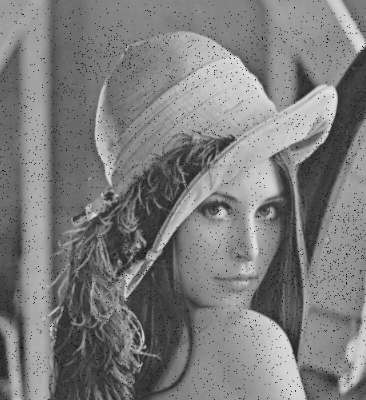
\includegraphics[width=\textwidth]{img/smooth-lena-input}
    \caption{Obraz wejściowy}
    \label{fig:smooth_lena_input}
  \end{subfigure}
  ~
  \begin{subfigure}[b]{0.45\textwidth}
    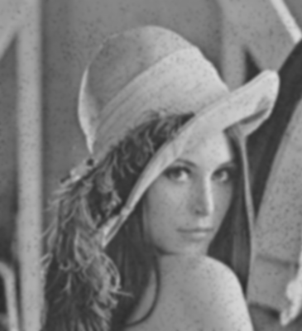
\includegraphics[width=\textwidth]{img/smooth-lena-gauss}
    \caption{Operacja rozmycia Gaussa}
    \label{fig:smooth_lena_gauss}
  \end{subfigure}
  ~
  \begin{subfigure}[b]{0.45\textwidth}
    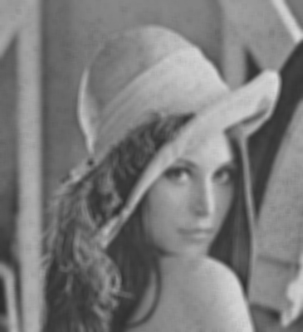
\includegraphics[width=\textwidth]{img/smooth-lena-mean}
    \caption{Operacja rozmycia średniego}
    \label{fig:smooth_lena_gauss}
  \end{subfigure}
  ~
  \begin{subfigure}[b]{0.45\textwidth}
    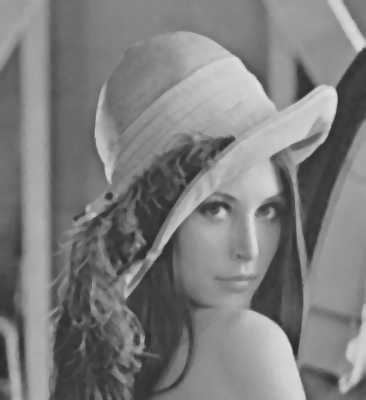
\includegraphics[width=\textwidth]{img/smooth-lena-median}
    \caption{Operacja rozmycia medianowego}
    \label{fig:smooth_lena_gauss}
  \end{subfigure}
  \caption{Wynik działania podstawowych operacji rozmycia na obrazie wejściowym}
  \label{fig:lena_smooth}
\end{figure}
\subsubsection{Dodawanie obrazów}
W tym podrozdziale, jako $n$ oznaczać będziemy liczbę obrazów wejściowych poddawanych operacji dodawania, jako $P^{(in)}_{i}$ będziemy rozumieć $i-ty$ obraz wejściowy, natomiast poprzez $f^{(in)}_i$ będziemy oznaczać funkcję $i-tego$ obrazu przyporządkowującą punktowi kolor. Symbolem $w_i$ będziemy oznaczać wagę przyporządkowaną do $i-tego$ obrazu wejściowego.\\
Operacja dodawania obrazów 
\begin{gather*}
P^{(out)} = P_1^{(in)} + P_2^{(in)} + ... + P_n^{(in)}
\end{gather*}
definiowana jest wzorem:
\begin{gather*}
  f^{(out)}(x, y) = \displaystyle\sum_{i=1}^{n} f^{(i)}(x, y), \quad (x, y) \in P^{(in)}_{N,M}.
\end{gather*}
\paragraph{Dodawanie obrazów z wagami} \mbox{}\\
Dodawanie obrazów z wagami zdefiniowane jest wzorem:
\begin{gather*}
  f^{(out)}(x, y) = \displaystyle\sum_{i=1}^{n} f^{(in)}_i(x, y) \cdot w_i, \quad (x, y) \in P^{(in)}_{N,M}.
\end{gather*}
\subsubsection{Wyostrzenie obrazu}
W celu uzyskania efektu wyostrzonych krawędzi obrazu, należy wykonać na obrazie wejściowym operację rozmycia Gaussa, a następnie obraz wynikowy dodać do obrazu wejściowego z wagami:
\begin{itemize}
  \item 1.5 dla obrazu wejściowego,
  \item -0.5 dla obrazu poddanego operacji rozmycia Gaussa.
\end{itemize}Na rysunku~\ref{fig:image_sharpen} przedstawiono obraz poddany operacji wyostrzania, oraz wynik tej operacji.
\begin{figure}
  \centering
  \begin{subfigure}[b]{0.45\textwidth}
    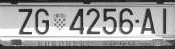
\includegraphics[width=\textwidth]{img/image-sharpen-before}
    \label{fig:image_sharpen_before}
  \end{subfigure}
  ~
  \begin{subfigure}[b]{0.45\textwidth}
    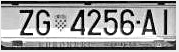
\includegraphics[width=\textwidth]{img/image-sharpen-after}
    \label{fig:image_sharpen_after}
  \end{subfigure}
  \caption{Operacja wyostrzenia wykonana na obrazie jednokanałowym}
  \label{fig:image_sharpen}
\end{figure}
\subsubsection{Normalizacja obrazu}
W tym podrozdziale jako $\min_{in}$ oraz $max_{in}$ będziemy oznaczać minimalną i maksymalną wartość funkcji jasności obrazu wejściowego, natomiast jako $\min_{out}$ oraz $min_{out}$ będziemy oznaczać minimalną i maksymalną pożądaną wartość funkcji jasności obrazu wyjściowego. \\
Operacja normalizacji służy do zmiany przedziału wartości pikseli występujących w obrazie, i definiowana jest wzorem:
\begin{gather*}
  f^{(out)}(x, y) = (f^{(in)}(x, y) - min_{in}) \cdot \frac{max_{out} - min_{out}}{max_{in} - min_{in}}+min_{in}, \quad \quad (x, y) \in P^{(in)}_{N,M}.
\end{gather*}
Rysunek~\ref{fig:image_normalize} prezentuje działanie algorytmu normalizacji. Obraz wejściowy został wykonany w bardzo ciemnym otoczeniu, natomiast po wykonaniu operacji kontrast obrazu został poprawiony.
\begin{figure}
  \centering
  \begin{subfigure}[b]{0.45\textwidth}
    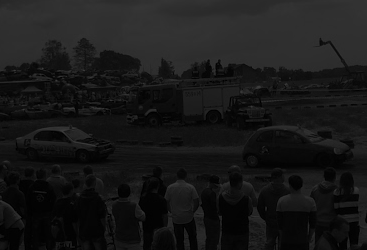
\includegraphics[width=\textwidth]{img/image-normalize-before}
    \label{fig:image_normalize_before}
  \end{subfigure}
  ~
  \begin{subfigure}[b]{0.45\textwidth}
    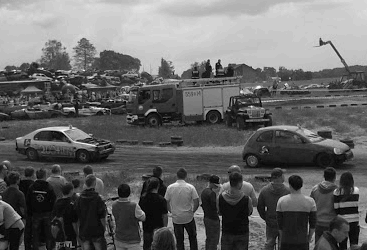
\includegraphics[width=\textwidth]{img/image-normalize-after}
    \label{fig:image_normalize_after}
  \end{subfigure}
  \caption{Normalizacja obrazu}
  \label{fig:image_normalize}
\end{figure}
\subsection{Operacje morfologiczne}
Operacje morfologiczne na obrazach wykorzystywane są do filtracji morfologicznej oraz analizy kształtów obiektów na obrazie. Definiują one zbiór punktów, jakie powinny pozostać na obrazie. W praktyce jest to realizowane poprzez ustawianie wartości jasności danego piksela na wartość 0 w przypadku nieistnienia danego punktu w zbiorze, lub wartości maksymalnej dla funkcji jasności, jeśli piksel o danych współrzędnych znajduje się w zbiorze. Przekształcenia morfologiczne są podstawą dla wielu bardziej złożonych algorytmów wizji komputerowej.\\
Jako symbol $A$ będziemy oznaczali zbiór punktów w których obraz wejściowy posiada wartość jasności równą 1, symbol $B$ będzie reprezentował maskę dla operacji morfologicznej. Funkcja $translacja(a, b)$ definiuje przesunięcie elementu strukturalnego (maski) $a$ na pozycję określoną przez współrzędne $b$.
\subsubsection{Dylatacja obrazu}
Dylatacja to rozszerzenie obrazu wykorzystując zadaną maskę. Operacja definiowana jest wzorem
\begin{gather*}
  A \oplus B \equiv \{ (x, y) \in A | A \cap translacja(B, (x, y)) \neq \emptyset \}.
\end{gather*}
Przykładowy wynik operacji dylatacji przedstawiony jest na rysunku~\ref{fig:dilate}.
\begin{figure}
  \centering
  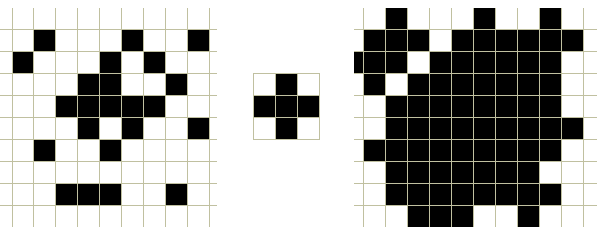
\includegraphics[width=15cm]{img/dilate}
  \caption{Obraz binarny poddany procesowi dylatacji z zadanym elementem strukturalnym}
  \label{fig:dilate}
\end{figure}
\subsubsection{Erozja obrazu} 
Erozja obrazu polega na zwężaniu obrazu z wykorzystaniem zadanego elementu strukturalnego. Operacja definiowana jest wzorem
\begin{gather*}
  A \ominus B \equiv \{ (x, y) \in A | translacja(B, (x, y) \subset A \}.
\end{gather*}
Przykładowy wynik operacji erozji obrazu przedstawiony został na rysunku~\ref{fig:erode}.
\begin{figure}
  \centering
  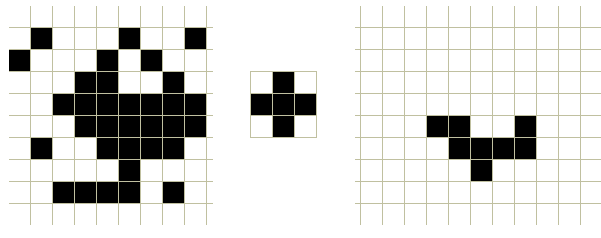
\includegraphics[width=15cm]{img/erode}
  \caption{Obraz binarny poddany procesowi erozji z zadanym elementem strukturalnym}
  \label{fig:erode}
\end{figure}
\subsubsection{Zamknięcie i otwarcie obrazu}
Operacje zamknięcia i otwarcia obrazu to złożenie dwóch wyżej wymienionych operacji (dylatacji oraz erozji) w odpowiedni sposób.
\begin{itemize}
\item zamknięcie obrazu definiowane jest w następujący sposób:
  \begin{gather*}
    A \bullet B = (A \oplus B) \ominus B,
  \end{gather*} 
czyli najpierw wykonywana jest operacja dylatacji obrazu, a następnie przekształcony obraz poddawany jest operacji erozji
\item otwarcie obrazu definiowane jest wzorem:
  \begin{gather*}
    A \circ B = (A \ominus B) \oplus B.
  \end{gather*}
W przypadku algorytmu otwarcia obrazu, w pierwszej kolejności wykonywana jest operacja erozji, a następnie operacja dylatacji obrazu.
\end{itemize}
Na rysunku~\ref{fig:open_close} przedstawiony został wynik działania obydwu algorytmów na tym samym obrazie, z tym samym elementem strukturalnym.
\begin{figure}
  \centering
  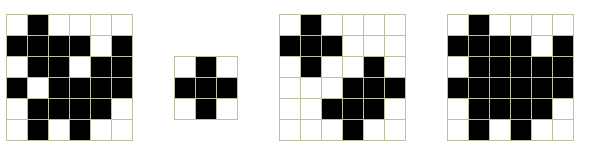
\includegraphics[width=15cm]{img/open-close}
  \caption{Obraz binarny poddany operacji otwarcia oraz zamknięcia obrazu, dla takiego samego elementu strukturalnego}
  \label{fig:open_close}
\end{figure}
\subsubsection{Transformata odległościowa}
Transformata odległościowa, inaczej zwana funkcją odległości, służy do wyznaczania minimalnej odległości punktu o wartości 1 od punktu o wartości 0. Dla punktów o wartości 0 automatycznie przypisywana jest wartość 0. \\
Tabela~\ref{tab:distance_transform} przedstawia wynik działania operacji na macierzy zawierającej obrazy binarne, natomiast rysunek~\ref{fig:distance_transform} prezentuje wynik działania tej samej operacji na obrazie. W celu podkreślenia wyniku operacji, obraz wyjściowy został poddany operacji normalizacji.

\begin{table}
\centering
\begin{minipage}[b]{80mm}
\centering
\begin{tabular}{|l|l|l|l|l|l|l|l|}
\hline
0&0&0&0&0&0&0&0 \\ \hline
0&1&1&1&1&1&1&0 \\ \hline
0&1&1&1&1&1&1&0 \\ \hline
0&1&1&1&1&1&1&0 \\ \hline
0&1&1&1&1&1&1&0 \\ \hline
0&1&1&1&1&1&1&0 \\ \hline
0&0&0&0&0&0&0&0 \\ \hline
\end{tabular}
\caption*{Binarny obraz wejściowy}
\end{minipage}
\begin{minipage}[b]{70mm}
\centering
\begin{tabular}{|l|l|l|l|l|l|l|l|}
\hline
0&0&0&0&0&0&0&0 \\ \hline
0&1&1&1&1&1&1&0 \\ \hline
0&1&2&2&2&2&1&0 \\ \hline
0&1&2&3&3&2&1&0 \\ \hline
0&1&2&2&2&2&1&0 \\ \hline
0&1&1&1&1&1&1&0 \\ \hline
0&0&0&0&0&0&0&0 \\ \hline
\end{tabular}
\caption*{Transformata odległościowa}
\end{minipage}
\caption{Transformacja odległościowa - macierz binarna} \label{tab:distance_transform} 
\end{table}

\begin{figure}
  \centering
  \begin{subfigure}[b]{0.45\textwidth}
    
\includegraphics[width=\textwidth]{img/distance-transform-before}
    \caption{Binarny obraz wejściowy}
    \label{fig:distance_transform_before}
  \end{subfigure}
  ~
  \begin{subfigure}[b]{0.45\textwidth}
    
\includegraphics[width=\textwidth]{img/distance-transform-after}
    \caption{Transformata odległościowa}
    \label{fig:distance_transform_after}
  \end{subfigure}
    \caption{Transformacja odległościowa - obraz binarny}
    \label{fig:distance_transform}
\end{figure}

\subsection{Operacje na histogramach}
Bardzo często podczas analizy obrazu pod kątem znajdowania segmentów, wykorzystywana jest analiza histogramu. W celu ułatwienia analizy, a także poprawy jej wyników, przed jej rozpoczęciem można zastosować niżej wymienione zabiegi.
\begin{figure}
  \centering
  \begin{subfigure}[b]{0.45\textwidth}
    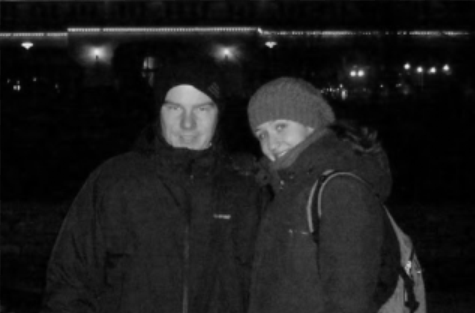
\includegraphics[width=\textwidth]{img/image-histogram}
    \label{fig:image_histogram}
  \end{subfigure}
  ~
  \begin{subfigure}[b]{0.45\textwidth}
    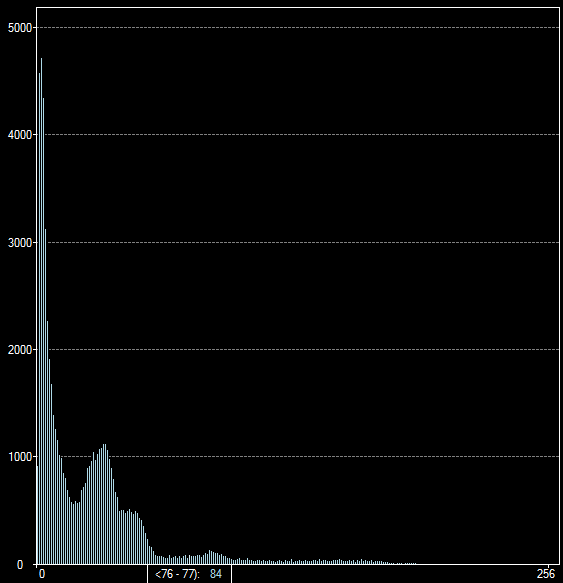
\includegraphics[width=\textwidth]{img/image-histogram-histogram}
    \label{fig:image_histogram_histogram}
  \end{subfigure}
  \caption{Jednokanałowy obraz oraz jego histogram}
  \label{fig:image_histogram_g}
\end{figure}
\textbf{Histogram obrazu} jest graficzną reprezentacją rozkładu częstości występowania danej wartości jasności w obrazie. Przykładowy obraz oraz jego histogram przedstawiony został na rysunku~\ref{fig:image_histogram_g}. Ponieważ obraz jest bardzo ciemny, większość wartości na histogramie jest bliska wartości 0 (ta wartość reprezentuje kolor czarny).\\
Jako $H$ będziemy oznaczali funkcję zwracającą wartość histogramu w podanym punkcie. Poprzez symbol $H_{max}$ oznaczać będziemy funkcję zwracającą największy indeks $i$ znajdujący się w histogramie, taki że $H(i) \neq 0$. Symbolem $H_{in}$ oznaczać będziemy histogram wejściowy, a symbolem $H_{out}$ histogram wyjściowy.\\

\subsubsection{Wyrównanie histogramu}
Metoda wyrównywania histogramu ma na celu zmianę kontrastu obrazu. Metoda ta wykorzystywany jest w przypadku, gdy zarówno tło, jak i pierwszy plan obrazu, są ciemne lub jasne. Wadą metody wyrównywania histogramu jest możliwe wzmocnienie zakłóceń występujących na obrazie, gdyż algorytm traktuje je jak sygnał opisujący prawidłowy obraz. Przed zastosowaniem tej metody, warto zatem zastosować jeden z algorytmów rozmycia obrazu, opisywany we wcześniejszej części tego rozdziału.\\
Metoda wyrównania histogramu sprowadza się do wyznaczenia tablicy LUT (\textit{ang. Lookup table}), na podstawie której wyznaczone zostaną wartości poszczególnych pikseli obrazu wejściowego. W celu wyznaczenia tablicy LUT, należy wyznaczyć dystrybuantę rozkładu prawdopodobieństwa dla wartości pikseli obrazu:
\begin{gather*}
  D(i) = \sum\limits_{j=0}^i p(j),
\end{gather*}
gdzie i jest wartością jasności występującą na obrazie, a p(j) jest prawdopodobieństwem wystąpienia wartości j w obrazie. Wykorzystując wyznaczone wartości dystrybuanty, możemy opisać tablicę LUT za pomocą wzoru:
\begin{gather*}
  LUT(i) = \frac{D(i)-D_0}{1-D_0} \cdot K,
\end{gather*}
gdzie i to wartość jasności składowej obrazu wejściowego, $D_0$ to pierwsza wartość dystrybuanty różna od zera, a K jest maksymalną wartością jasności występującym w obrazie wejściowym.\\
Rysunek~\ref{fig:equalize_histogram} przedstawia efekt działania operacji wyrównania histogramu na przykładowym obrazie.
\begin{figure}
  \centering
  \begin{subfigure}[b]{0.45\textwidth}
    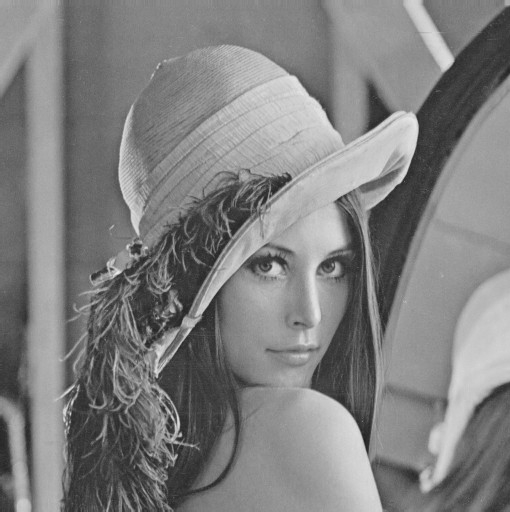
\includegraphics[width=\textwidth]{img/equalize-histogram-before}
    \caption{Obraz wejściowy dla operacji wyrównania histogramu}
    \label{fig:equalize_histogram_before}
  \end{subfigure}
  ~
  \begin{subfigure}[b]{0.45\textwidth}
    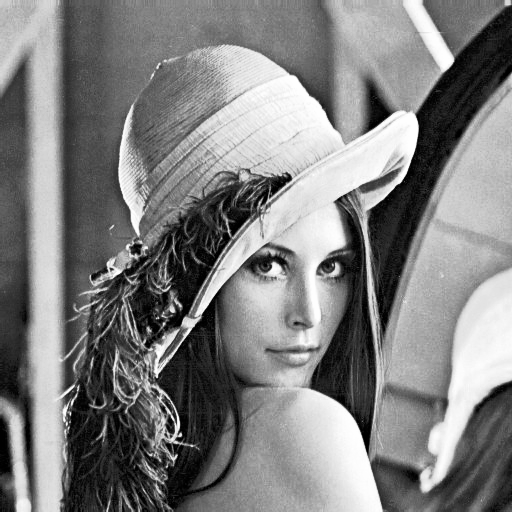
\includegraphics[width=\textwidth]{img/equalize-histogram-after}
    \caption{Obraz wyjściowy, poddany operacji wyrównania histogramu}
    \label{fig:equalize_histogram_after}
  \end{subfigure}
  ~
  \begin{subfigure}[b]{0.45\textwidth}
    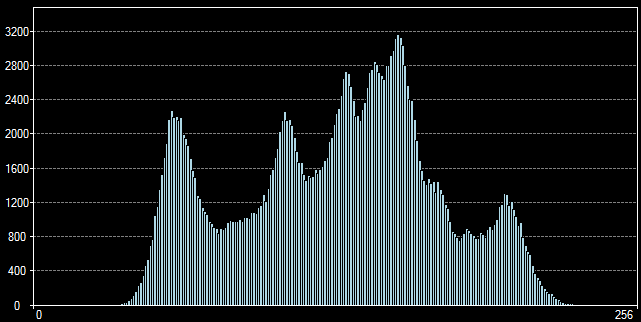
\includegraphics[width=\textwidth]{img/equalize-histogram-histogram-before}
    \caption{Histogram obrazu wejściowego}
    \label{fig:equalize_histogram_histogram_before}
  \end{subfigure}
  ~
  \begin{subfigure}[b]{0.45\textwidth}
    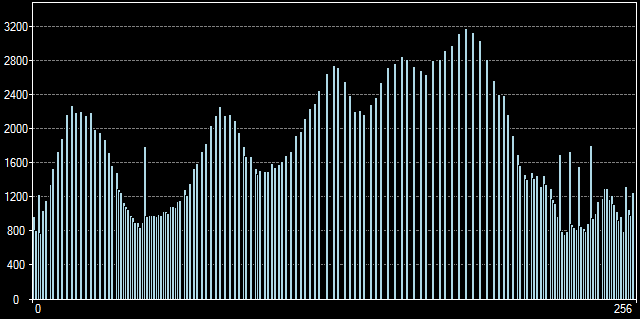
\includegraphics[width=\textwidth]{img/equalize-histogram-histogram-after}
    \caption{Histogram obrazu wyjściowego}
    \label{fig:equalize_histogram_histogram_after}
  \end{subfigure}
  \caption{Operacja wyrównania histogramu dla obrazu jednokanałowego}\label{fig:equalize_histogram}
\end{figure}

\subsubsection{Wygładzenie histogramu}
Często histogram obrazu zawiera w sobie nagłe skoki wartości, które utrudniają analizę histogramu, gdyż mogą reprezentować fałszywe ekstrema. Wygładzanie histogramu ma na celu usunięcie takich skoków, zachowując przy tym oryginalny kształt histogramu. Dla każdej wartości histogramu wejściowego \textit{$H_{in}$} należy zastosować następującą operację:
\begin{gather*}
  \forall_{i} \in \big< H_{in}(0), H_{in}(H_{max}(H_{in})) \big> :  H_{out}(i) = \frac{H_{in}(i-1) + H_{in}(i) + H_{in}(i+1)}{3}.
\end{gather*}
Przykład działania algorytmu wygładzania histogramu przedstawiony został na rysunku~\ref{fig:histogram_smooth}.
\begin{figure}
  \centering
  \begin{subfigure}[b]{0.45\textwidth}
    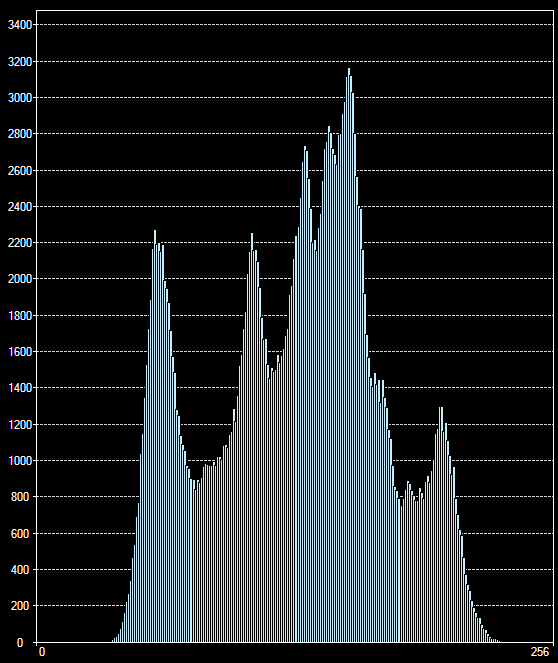
\includegraphics[width=\textwidth]{img/smooth-histogram-before}
    \caption{Obraz wejściowy dla operacji wygładzenia histogramu}
    \label{fig:equalize_histogram_before}
  \end{subfigure}
  ~
  \begin{subfigure}[b]{0.45\textwidth}
    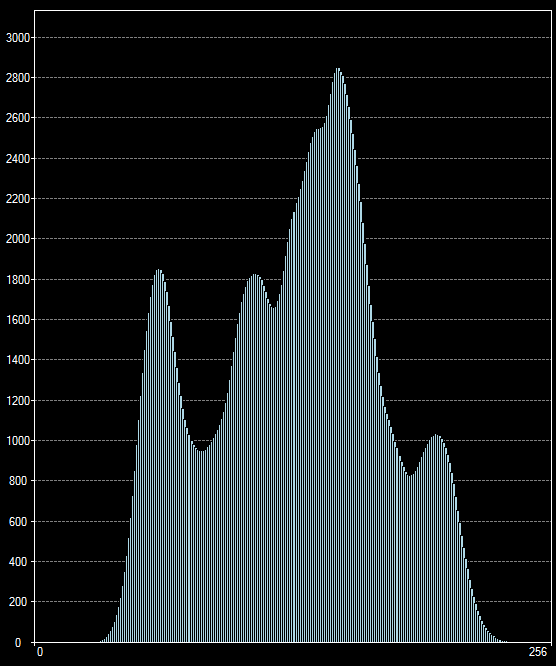
\includegraphics[width=\textwidth]{img/smooth-histogram-after}
    \caption{Obraz wyjściowy, poddany operacji wygładzenia histogramu}
    \label{fig:equalize_histogram_after}
  \end{subfigure}
  \caption{Operacja wygładzenia histogramu}\label{fig:histogram_smooth}
\end{figure}

\newpage
\cite{foo}

\bibliographystyle{plain}
\bibliography{main_document}

\end{document}
